%%
%% This is file `chapmin.tex',
%% generated with the docstrip utility.
%%
%% The original source files were:
%%
%% ths.dtx  (with options: `chapmin')
%% 
%% IMPORTANT NOTICE:
%% 
%% For the copyright see the source file.
%% 
%% Any modified versions of this file must be renamed
%% with new filenames distinct from chapmin.tex.
%% 
%% For distribution of the original source see the terms
%% for copying and modification in the file ths.dtx.
%% 
%% This generated file may be distributed as long as the
%% original source files, as listed above, are part of the
%% same distribution. (The sources need not necessarily be
%% in the same archive or directory.)


\section{Mathmatic Development}

Where does this text go?

\subsection{The Boltzmann Equation}

The time dependent gamma transport equation can be written as

\begin{equation} \label{eq:boltz_t_dep}
\begin{split}
	&\left[ \frac{1}{v(E)} \frac{\partial}{\partial t} + \hat{\Omega} \cdot \nabla + \Sigma_t(\boldsymbol{r}, E, t) \right]
	\psi(\boldsymbol{r}, E, \hat{\Omega}, t) = \\
	&\int_{4 \pi} \int_0^\infty \Sigma_s(\boldsymbol{r}, E' \rightarrow E, \hat{\Omega}' \rightarrow \hat{\Omega}, t) \psi(\boldsymbol{r}, E', \hat{\Omega}', t) dE' d\hat{\Omega}' + S(\boldsymbol{r}, E, \hat{\Omega}, t)
\end{split}
\end{equation}

However, we are typically not concerned with the transient case in medical diagnostic imaging. We are more interested in the steady state case. The time independent form of Eq. \ref{eq:boltz_t_dep} is written as

\begin{equation} \label{eq:boltz}
\begin{split}
	&\left[ \hat{\Omega} \cdot \nabla + \Sigma_t(\boldsymbol{r}, E) \right]
	\psi(\boldsymbol{r}, E, \hat{\Omega}) = \\
	&\int_{4 \pi} \int_0^\infty \Sigma_s(\boldsymbol{r}, E' \rightarrow E, \hat{\Omega}' \rightarrow \hat{\Omega}) \psi(\boldsymbol{r}, E', \hat{\Omega}') dE' d\hat{\Omega}' + S(\boldsymbol{r}, E, \hat{\Omega})
\end{split}
\end{equation}

The following sections show how Eq.~\ref{eq:boltz} is discretized.

\subsection{Angular Discretization}
The coordinate system used in DOCTORS is shown in Fig.~\ref{fig:coord_sys}. A discrete set of $N_a$ angles ($\Omega_{a} \quad a = 0 \ldots N_a-1$) is selected to represent continuous directional space. Particles are transported only along these discrete directions form one voxel to adjacent voxels.

The rotation symmetrical quadrature is implemented in DOCTORS. There are many different quadrature sets, the rotation symmetrical quadratures were selected because they are easy to implement, rotationally symmetric, and the most commonly used in production discrete ordinate solvers. This enables simple, direct comparison to other solvers. Arbitrary quadratures are permissible in a plain text file supplied by the user enabling other quadratures.

\begin{figure}[tb]
  \begin{center}
   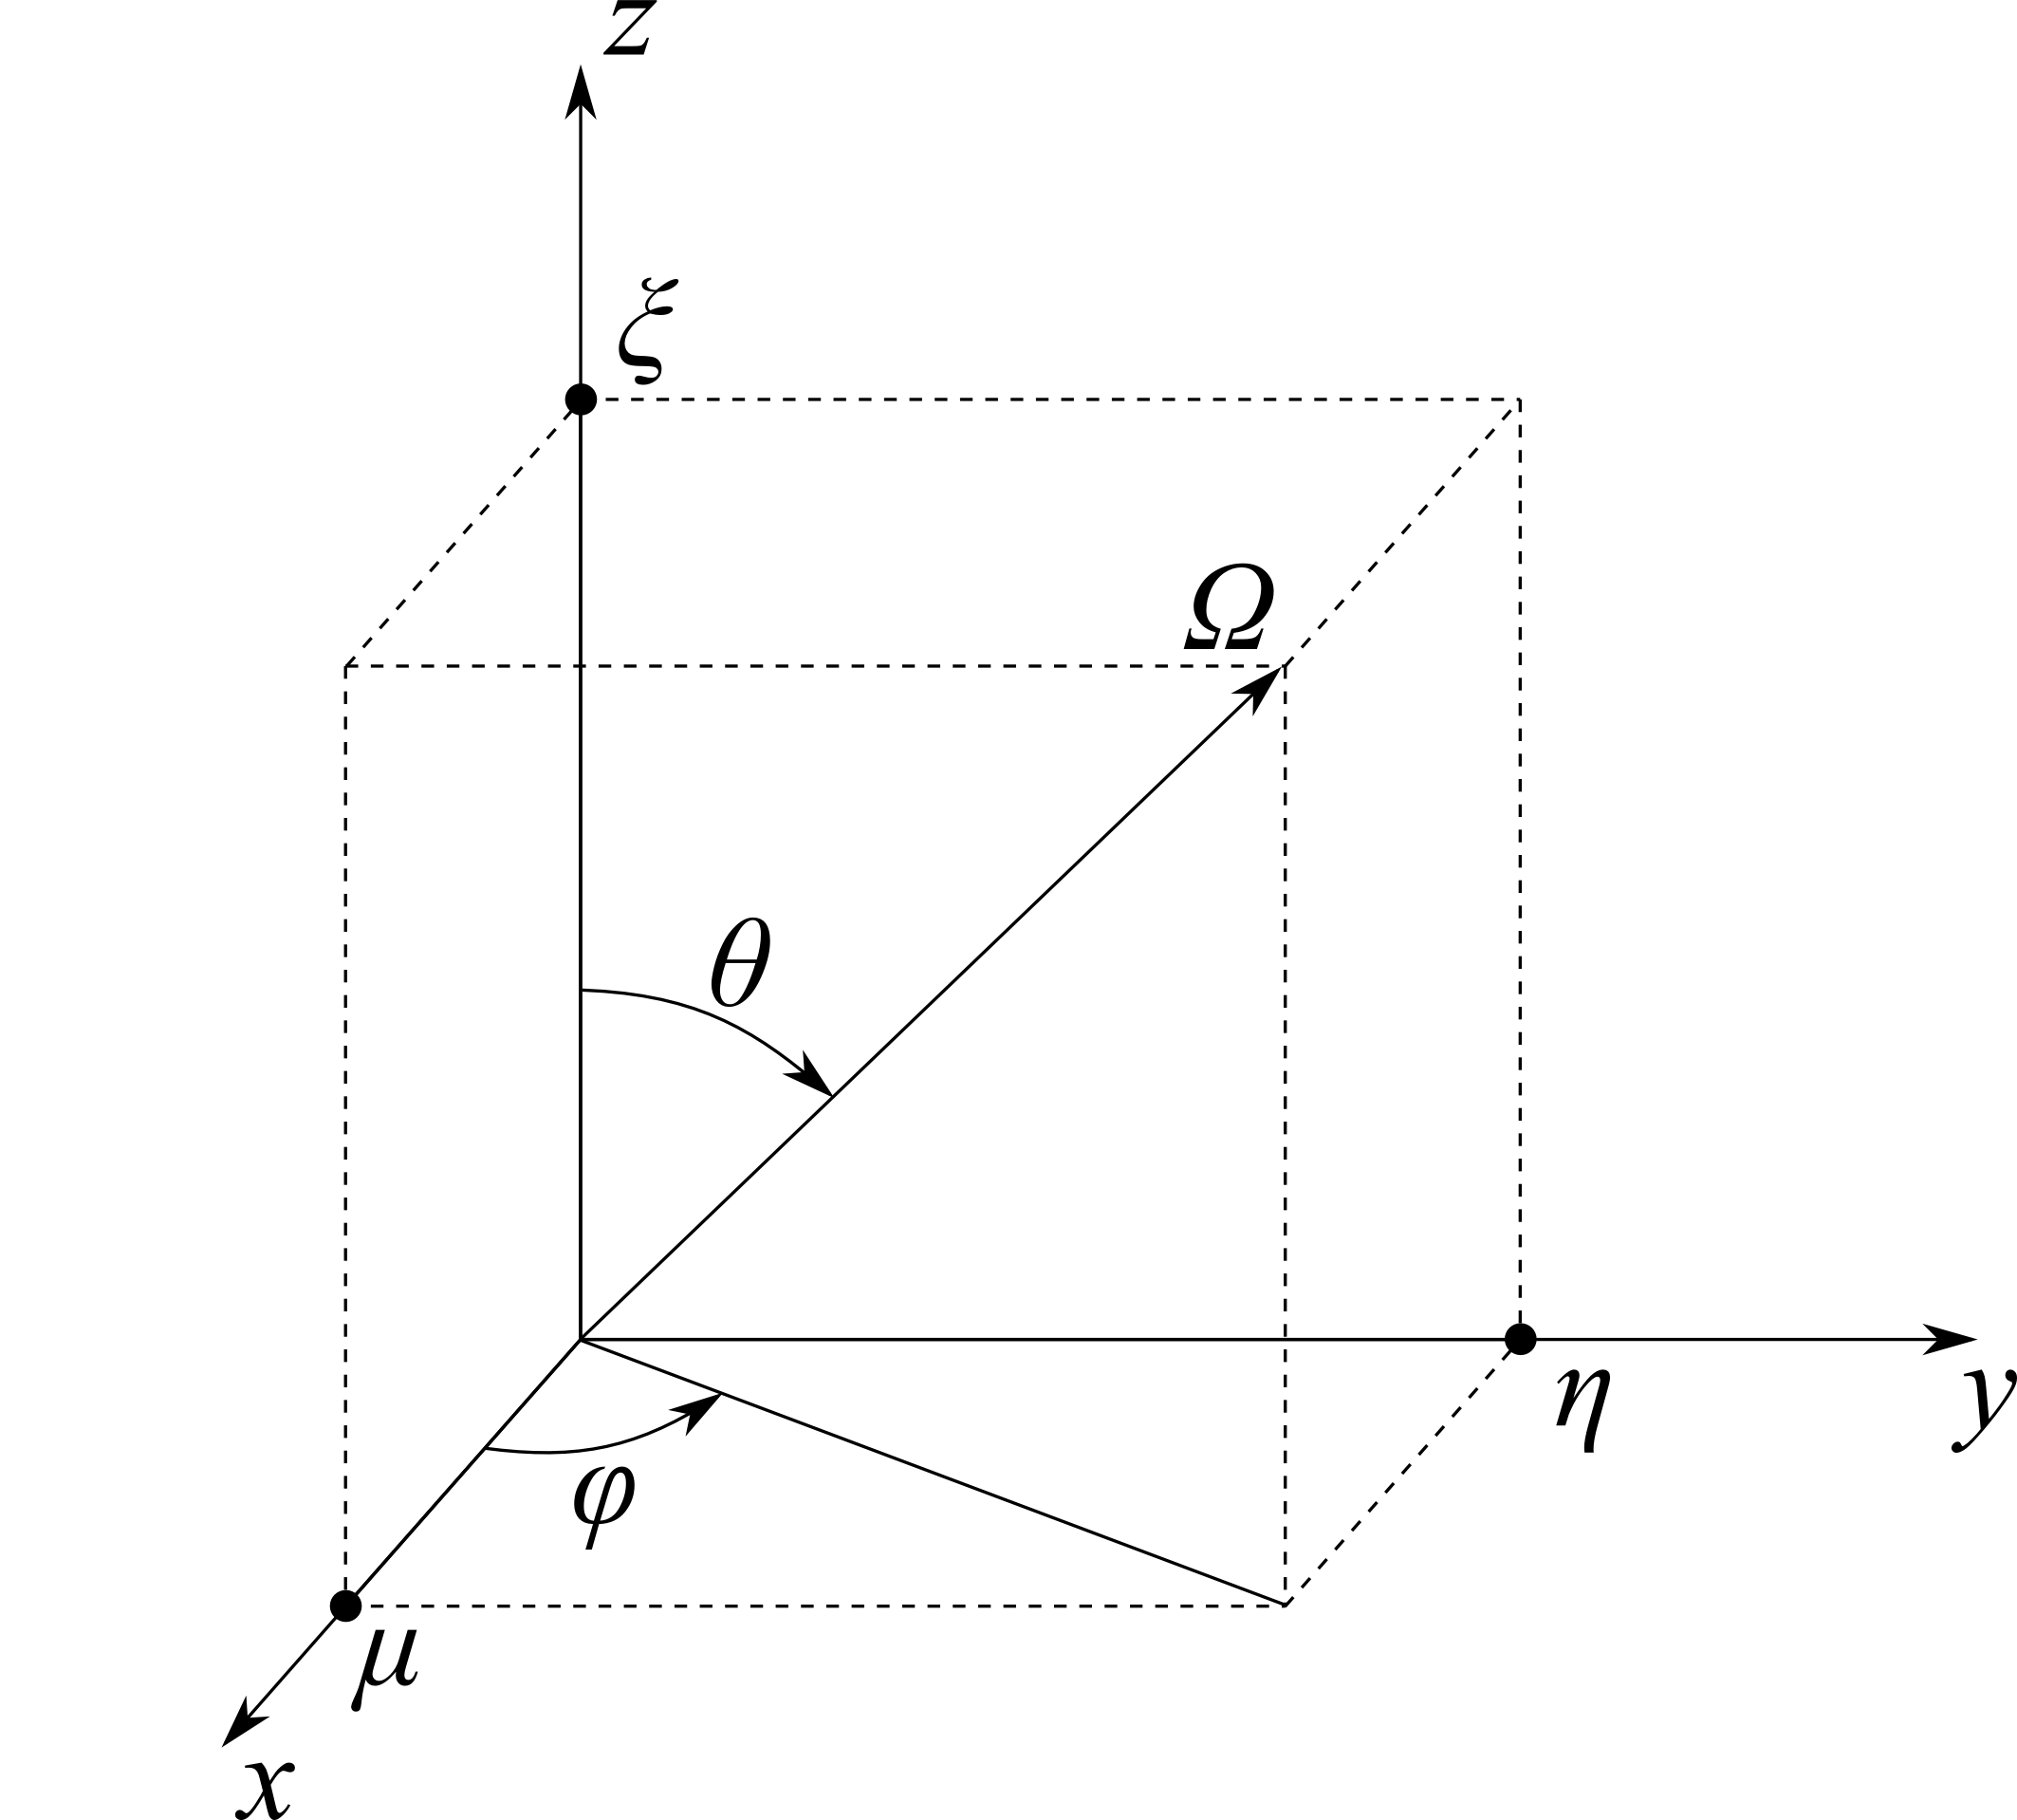
\includegraphics[width=3.75in]{figs/coord_sys}
  \end{center}
  \caption{The coordinate system used in DOCTORS. Given an arbitrary direction, $\Omega$, $\mu$, $\eta$, and $\xi$ are its direction cosines with respect to the $x$, $y$, and $z$ axes respectively. $\varphi$ is the azimuthal angle (with respect to $x$ and the d $\theta$ is the polar angle (with respect to $z$).}
\label{fig:coord_sys}
\end{figure}%

A given direction, $\hat{\Omega}$ is determined by its three cosine components. This relation is given in Eq.~\ref{eq:omega_cos} where $\hat{i}$, $\hat{j}$, and $\hat{k}$ are the unit directions in the $x$, $y$, and $z$ directions respectively.

\begin{equation} \label{eq:omega_cos}
	\hat{\Omega} = \mu \hat{i} + \eta \hat{j} + \xi \hat{k}
\end{equation}

Each discrete angle is associated a weight. The weights are designed with the angles such that once a discrete quadrature is selected, integration over continuous space becomes integration in discrete space approximated by Eq.~\ref{eq:disc_int}.

\begin{equation} \label{eq:disc_int}
\int_{4 \pi} f(\hat{\Omega}) d\Omega \approx \sum_{a=0}^{N_a-1} f(\hat{\Omega}_a) \omega_a
\end{equation}

Discretizing Eq.~\ref{eq:boltz} in angular space gives Eq.~\ref{eq:boltz_a} where the angle is denoted by subscript $a$.

\begin{equation} \label{eq:boltz_a}
\begin{split}
&\left[ \hat{\Omega}_a \cdot \nabla + \Sigma_t(\boldsymbol{r}, E) \right]
\psi_{a}(\boldsymbol{r}, E) = \\
&\sum_{a=0}^{N_a-1} \int_0^\infty \Sigma_{s, a, a'}(\boldsymbol{r}, E' \rightarrow E) \psi_{a'}(\boldsymbol{r}, E') dE' \omega_a + S_a(\boldsymbol{r}, E)
\end{split}
\end{equation}

\subsection{Energy Discretization}

Continuous energy is discretized into $G$ groups indexed from 0 to $G-1$. Upscatter is assumed to be negligible. Therefore, Eq.~\ref{eq:boltz_a} becomes the energy discretized Eq.~\ref{eq:boltz_e} where the group number is indexed by superscript $g$. The group structure is shown in Fig.~\ref{fig:energy_groups}.

\begin{equation} \label{eq:boltz_e}
\left[ \hat{\Omega}_a \cdot \nabla + \Sigma_t^g(\boldsymbol{r}) \right]
\psi_{a}^{g}(\boldsymbol{r}) = 
\sum_{a=0}^{N_a-1} \sum_{g'=g}^{G-1} \Sigma_{s, a, a'}^{g, g'}(\boldsymbol{r}) \psi_{a'}^{g'}(\boldsymbol{r}) \omega_a + S_a^g(\boldsymbol{r})
\end{equation}

\begin{figure}[tb]
  \begin{center}
   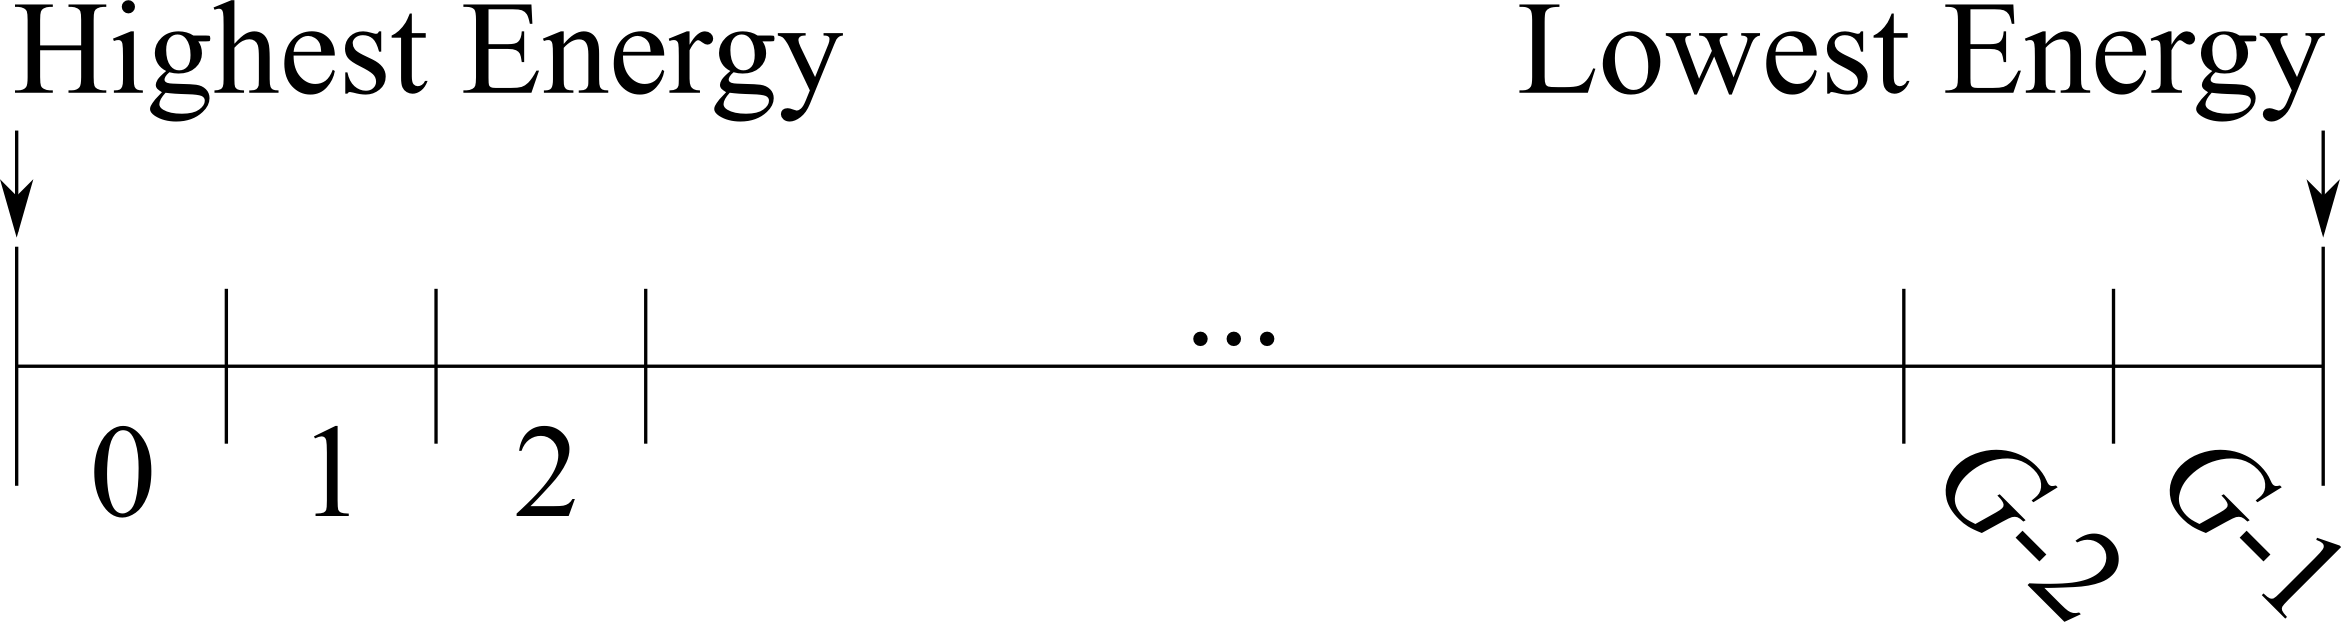
\includegraphics[width=3.75in]{figs/energy_groups}
  \end{center}
  \caption{The energy grid structure used in DOCTORS. The highest energy group is group 0 and the lowest energy is group $G-1$.}
\label{fig:energy_groups}
\end{figure}

The energy group structure should be selected appropriately for the problem.

The cross sections currently availabl eare those available from the SCALE 6.2 distribution. Those cross sections are designed for light water reactor analysis and are not well suited to medical physics applications. This is currently one of the greatest limitaitons of DOCOTRS. The SCALE cross section data also contains neutron data which is useless for the CT dosimetry DOCTORS performs.

Once the energy group structure is selected, cross section data must be available. Group averaged cross section values from energy $E_1$ to $E_2$ are computed using Eq.~\ref{eq:groupxs} where $\sigma(E)$ is the continuous microscopic cross section. A weighting function, $f$, is used to weight some energies. The weighting function can be any of a number commonly used functions. The following section discusses the data format used by the DOCTORS code.

\begin{equation}\label{eq:groupxs}
\sigma_G = \frac{\int_{E_1}^{E_2}f(E')\sigma(E') dE'}{\int_{E_1}^{E_2}}
\end{equation}

\subsection{Cross Section Parsing}
AMPX cross sections are read in binary. They are formatted like so. They are read like so. They were obtained from SCALE6.2. These files can be generated by other codes.

The file is split into a series of records. Each record is a string of binary bytes between a four byte header and four byte footer. The header and footer are identical and, when interpreted as a signed four byte integer, give the size in words of the record. A word is a 32-bit chunk (4 bytes) of binary data. The data is stored in Big Endian format which must be converted to Little Endian for most Intel and AMD processors. An example record is shown in Fig.~\ref{fig:ampxbytes1} and the endianess rearrangement is shown in Fig.~\ref{fig:ampxbytes2}. Once the bytes are properly ordered, the entire string can be reinterpreted as a 32-bit integer. In the case of the header bytes given in Fig.~\ref{fig:ampxbytes1} and~\ref{fig:ampxbytes2}, the bytes correspond to the integer 440 which is the length in bytes of the header record.

\begin{figure}[tb]
  \begin{center}
   \includegraphics[width=3.75in]{figs/ampxbytes1}
  \end{center}
  \caption{The bytes}
\label{fig:ampxbytes1}
\end{figure}

\begin{figure}[tb]
  \begin{center}
   \includegraphics[width=3.75in]{figs/ampxbytes2}
  \end{center}
  \caption{The byte ordering.}
\label{fig:ampxbytes2}
\end{figure}

The size always reports the number of 32-bit words required to store the data. However, some data types, such as characters, are only 8 bits so each word represents four distinct characters.

DOCTORS reads AMPX fromatted binary data files. Figure~\ref{fig:ampx} shows the data format of the overall file. The header section contains information about each individual nuclide such as which reaction types are available as well as information the same such as the group structure information.

The first entry in a nuclide is the directory record. The directory contains general information regarding the nuclide and information necessary to parse the proceeding records.

Bondarenko data and resonance parameters.

The next block of data contains the average cross section data. This data is averaged over all energies and directions using Eq.~\ref{eq:groupxs}. The only data used in this section in DOCTORS is the total cross section values necessary for implementing the fully discretized form of the LBE given later.

The 2D data is stored in a special format optimized for scatter matrix data.

\begin{figure}
    \centering
    \begin{subfigure}[b]{0.45\textwidth}
        \includegraphics[width=\textwidth]{figs/ampx1}
        \caption{The AMPX file format}
        \label{fig:ampx1}
    \end{subfigure}
    ~
    \begin{subfigure}[b]{0.45\textwidth}
        \includegraphics[width=\textwidth]{figs/ampx2}
        \caption{The structure of each individual record.}
        \label{fig:ampx2}
    \end{subfigure}
    \caption{The format of the AMPX file.}\label{fig:ampx}
\end{figure}

The binary data file is composed of multiple records, each of one of thirteen types. Each record is formatted differently to hold different data.

\subsection{Spatial Discretization}

Finally, Eq.~\ref{eq:boltz_e} is discretized in space to give Eq.~\ref{eq:boltz_i} which is fully discretized. The problem domain is split into an evenly spaced Cartesian grid. The grid spacing between each of the spatial dimensions does not necessarily need to be uniform, but it often is in the case of CT voxel phantoms.

The problem domain must be a regular rectangular parallelpiped of size $D_x$, $D_y$, and $D_z$ in the $x$, $y$, and $z$ directions respectively. The mesh is partitioned into $N_x$, $N_y$, and $N_z$ evenly spaced bins along each direction. The total number of voxels, $N_V$ is easily computed as the multiple of each of the component directions given in Eq.~\ref{eq:n_v}.

\begin{equation} \label{eq:n_v}
	N_V = N_x N_y N_z
\end{equation}

Voxel indices are reordered into a one dimensional vector (flattened) according to the rule given in Eq.~\ref{eq:indx_flat}. Note that indices start at zero.

\begin{equation} \label{eq:indx_flat}
	i = i_x (N_z + N_y) + i_y N_z + i_z
\end{equation}

The spatial mesh is shown in Fig.~\ref{fig:spatial_disc}. The size of each voxel in each dimension is computed by dividing the size of the problem domain along in that dimension by the number of mesh elements along the same direction. Eq.~\ref{eq:mesh_x} shows this computation for the $x$ direction. Analagous equations apply in the $y$ and $z$ directions as well.

\begin{equation} \label{eq:mesh_x}
\Delta x = \frac{D_x}{N_x}
\end{equation}

\begin{figure}[tb]
  \begin{center}
   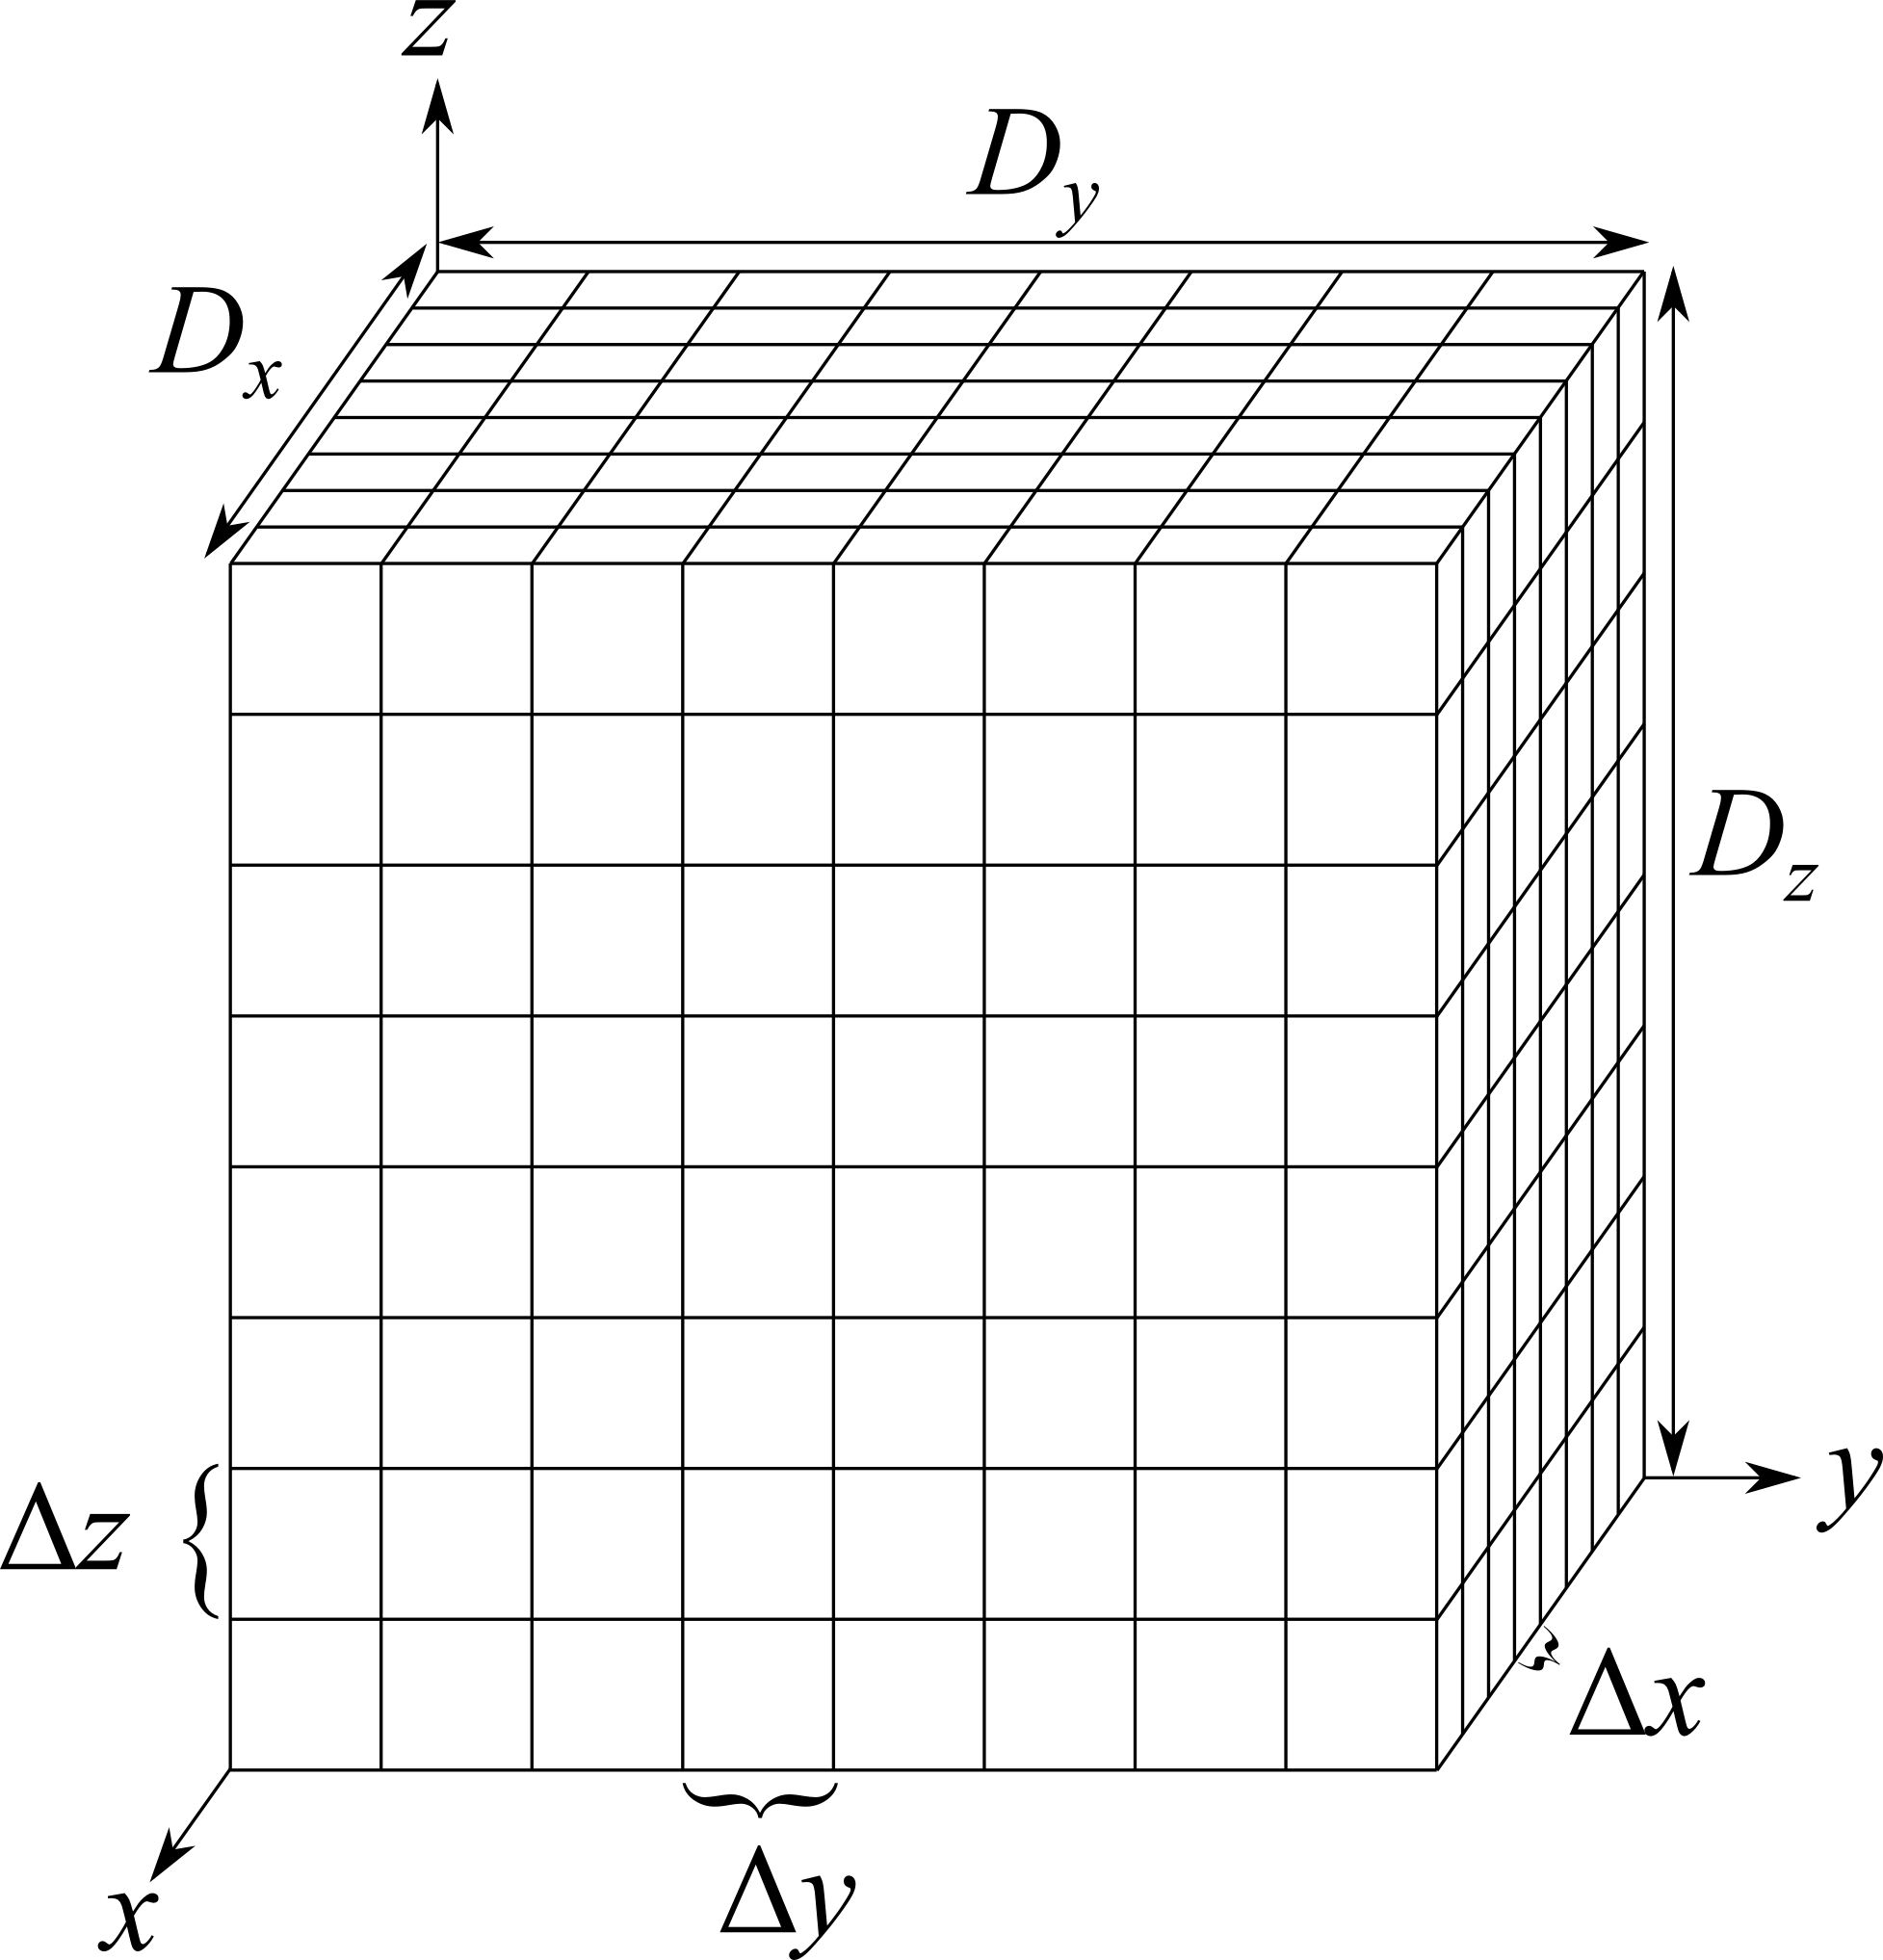
\includegraphics[width=3.75in]{figs/spatial_disc}
  \end{center}
  \caption{The spatial mesh imposed on the problem domain.}
\label{fig:spatial_disc}
\end{figure}

The index of interest is denoted as a subscript $i$ which makes the fully discretized form of the steady state Linear Boltzmann Equation given in Eq.~\ref{eq:boltz} into the fully discretized form given in Eq.~\ref{eq:boltz_i}

\begin{equation} \label{eq:boltz_i}
\left[ \hat{\Omega}_a \cdot \nabla + \Sigma_{t,i}^g \right]
\psi_{i,a}^{g} = 
\sum_{a=0}^{N_a-1} \sum_{g'=g}^{G-1} \Sigma_{s, i, a, a'}^{g, g'} \psi_{i, a'}^{g'} \omega_a + S_{i,a}^g
\end{equation}

\subsection{Solution}

To solve the fully discretized form of the Linear Boltzmann Equation given in Eq.~\ref{eq:boltz_i}, the gradient operator must first be computed numerically. Recall that $\Omega_a$ can be written in vector notation using its cosine components as defined in Eq.~\ref{eq:omega_cos}. Also recall the definition of the gradient, given in Eq.~\ref{eq:grad}.

\begin{equation} \label{eq:grad}
\nabla f(x, y, z) = \frac{\partial f(x, y, z)}{\partial x} \hat{i} + \frac{\partial f(x, y, z)}{\partial y} \hat{j} + \frac{\partial f(x, y, z)}{\partial z} \hat{k}
\end{equation}

To the first order, a partial derivitive can be computed using Eq.~\ref{eq:deriv_1}.

\begin{equation} \label{eq:deriv_1}
\frac{\partial f(x)}{\partial x} \approx \frac{f(x) - f(x + \Delta x)}{\Delta x}
\end{equation}

Using the definition of $\Omega$ and Eq.~\ref{eq:grad} the $\hat{\Omega} \cdot \nabla \psi$ term can be rewritten using Eq.~\ref{eq:spatial_1}

\begin{equation} \label{eq:spatial_1}
\begin{split}
\Omega \cdot \nabla \psi & \approx 
\left\langle \mu, \eta, \xi \right\rangle \cdot
\left\langle \frac{\psi(x) - \psi(x + \Delta x)}{\Delta x},
\frac{\psi(y + \Delta y) - \psi(y)}{\Delta y},
\frac{\psi(z + \Delta z) - \psi(z)}{\Delta z} \right\rangle \\
& \approx 
\frac{\psi(x + \Delta x) - \psi(x)}{\Delta x} \mu + 
\frac{\psi(y + \Delta y) - \psi(y)}{\Delta y} \eta + 
\frac{\psi(z + \Delta z) - \psi(z)}{\Delta z} \xi
\end{split}
\end{equation}

Along some direction, $\Omega$, as it enters an arbitrary voxel, it must pass through either of the sides indicated in red and exit via the other as shown in Fig.~\ref{fig:gradient}. Fig.~\ref{fig:gradient} uses the $yz$ faces of the voxel for illustration. If $\eta$ is positive, $\Omega$ will enter through the $x_i$ surface and exit through the $x_{i+1}$ surface. If $\eta$ is negative, this order will be reversed. A limitation to this methodology is that $\mu$, $\eta$, and $\xi$ are assumed to be nonzero. This is ensured as long as none of the directions in the quadrature are parallel to a major axis.

\begin{figure}[tb]
  \begin{center}
   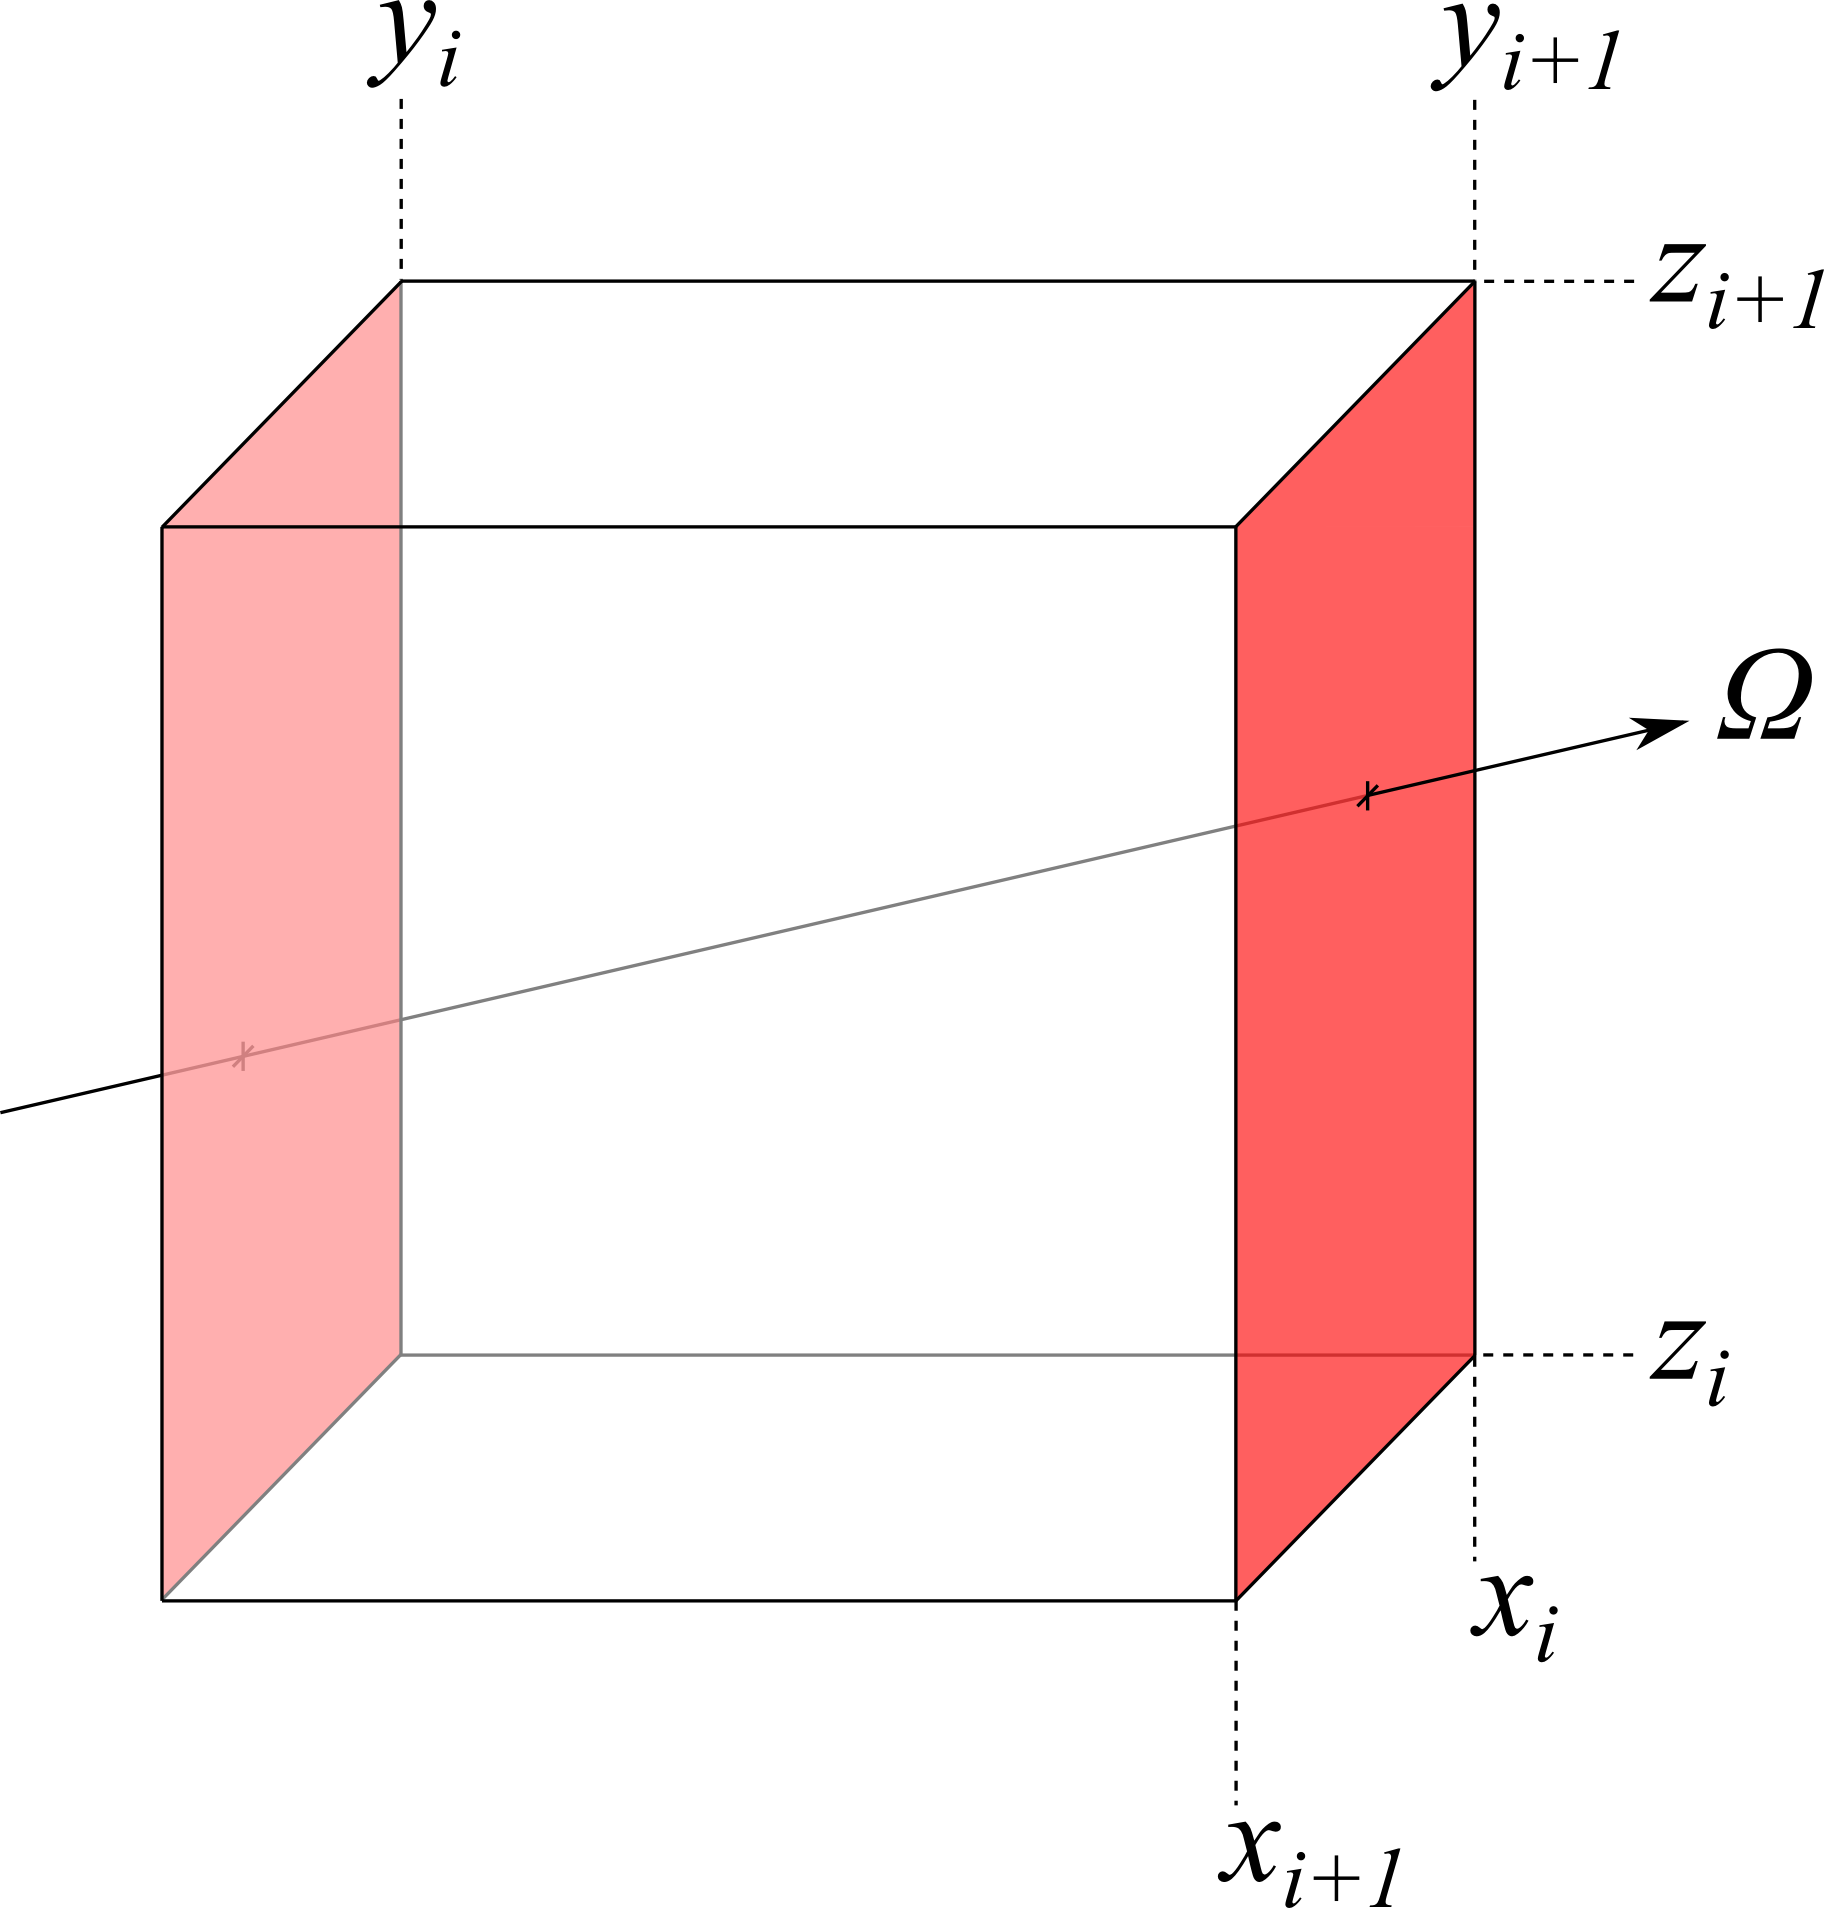
\includegraphics[width=3.75in]{figs/gradient}
  \end{center}
  \caption{The caption.}
\label{fig:gradient}
\end{figure}%

Depending on the sign of $\eta$, the first order approximation of the a derivitive along the $y$ direction is given by Eq.~\ref{eq:grad_y}.

\begin{equation} \label{eq:grad_y}
\begin{split}
\frac{\partial f}{\partial y} &= \frac{f(x_i) - f(x_{i+1})}{\Delta x}, \quad \eta>0 \\
\frac{\partial f}{\partial y} &= \frac{f(x_{i+1}) - f(x_{i})}{\Delta x}, \quad \eta <0 \\
\frac{\partial f}{\partial y} &= 0, \quad \eta=0
\end{split}
\end{equation}

Equation~\ref{eq:grad_y} can be generalized to use $f_{in}$ and $f_{out}$ instead of relying on the $x$-coordinate. This is given in Eq.~\ref{eq:grad_y2}

\begin{equation} \label{eq:grad_y2}
\begin{split}
\frac{\partial f}{\partial y} &= \frac{f_{in} - f_{out}}{\Delta x}, \quad \eta \neq 0 \\
\frac{\partial f}{\partial y} &= 0, \quad \eta=0
\end{split}
\end{equation}

The generalization of Eq.~\ref{eq:grad_y2} is applied to Eq.~\ref{eq:deriv_1} to yield Eq.~\ref{eq:deriv_2} which is generally valid for all octants.

\begin{equation} \label{eq:deriv_2}
\Omega \cdot \nabla \psi \approx 
\frac{\psi_{x,in} - \psi_{x,out}}{\Delta x} \mu + 
\frac{\psi_{y,in} - \psi_{y,out}}{\Delta y} \eta + 
\frac{\psi_{z,in} - \psi_{z,out}}{\Delta z} \xi
\end{equation}

Using the approximation given in Eq.~\ref{eq:deriv_2}, Eq.~\ref{eq:boltz_i} can be rewritten as Eq.~\ref{eq:boltz_i2}.

\begin{equation} \label{eq:boltz_i2}
\left[ 
\frac{\psi_{i,a,x,in}^g - \psi_{i,a,x,out}^g}{\Delta x} \mu + 
\frac{\psi_{i,a,y,in}^g - \psi_{i,a,y,out}^g}{\Delta y} \eta + 
\frac{\psi_{i,a,z,in}^g - \psi_{i,a,z,out}^g}{\Delta z} \xi
\right]
+ \Sigma_{t,i}^g \psi_{i,a}^{g} = 
\sum_{a=0}^{N_a-1} \sum_{g'=g}^{G-1} \Sigma_{s, i, a, a'}^{g, g'} \psi_{i, a'}^{g'} \omega_a + S_{i,a}^g
\end{equation}

It is useful to point out that each of $\psi_{i,a,x,in}^g$, $\psi_{i,a,x,out}^g$, $\psi_{i,a,y,in}^g$, $\psi_{i,a,y,out}^g$, $\psi_{i,a,z,in}^g$, and $\psi_{i,a,z,out}^g$ are \textit{surface} flux values while $\psi_{i,a}^{g}$ is a \textit{volume averaged} flux value.

In order for the discretized Linear Boltzmann Equation to be solved using Eq.~\ref{eq:boltz_i2}, the incoming flux must always be known. Either the boundary conditions or previously calculated values are used to determine each incoming flux. Therefore, in order to compute the average flux in a cell, some relationship between the average flux and the outgoing surface fluxes must be known. These values can be related by any one of many different mechanisms, the most common of which is the diamond difference approximation.

\subsection{Diamond Difference Approximation}

In the diamond difference approximation, it is assumed that the incoming and outgoing flux are both known. The average flux is assumed to be the average of the two surface fluxes. This is assumed to be the case in all three spatial dimensions. This leads to Eq.~\ref{eq:dd}.

\begin{equation} \label{eq:dd}
\begin{split}
\frac{\psi_{i,a,x,in}^g + \psi_{i,a,x,out}^g}{2} &= \psi_{i,a}^{g} \\
\frac{\psi_{i,a,y,in}^g + \psi_{i,a,y,out}^g}{2} &= \psi_{i,a}^{g} \\
\frac{\psi_{i,a,z,in}^g + \psi_{i,a,z,out}^g}{2} &= \psi_{i,a}^{g}
\end{split}
\end{equation}

Multiplying both sides of Eq.~\ref{eq:dd} and subtracting twice the outgoing surface flux from each yields Eq.~\ref{eq:dd2}.

\begin{equation} \label{eq:dd2}
\begin{split}
\psi_{i,a,x,in}^g - \psi_{i,a,x,out}^g &= 2\psi_{i,a}^{g} - \psi_{i,a,x,out}^g \\
\psi_{i,a,y,in}^g - \psi_{i,a,y,out}^g &= 2\psi_{i,a}^{g} - \psi_{i,a,y,out}^g \\
\psi_{i,a,z,in}^g - \psi_{i,a,z,out}^g &= 2\psi_{i,a}^{g} - \psi_{i,a,z,out}^g
\end{split}
\end{equation}

The form of the left hand side of Eq.~\ref{eq:dd2} is the same as in Eq.~\ref{eq:boltz_i2}. This allows Eq.~\ref{eq:dd2} to be used to make a substitution in Eq.~\ref{eq:boltz_i2} that removes the dependence on the outgoing flux from discretized equation. After the substitution, Eq.~\ref{eq:boltz_i3} will arise.

\begin{equation} \label{eq:boltz_i3}
\left[ 
\frac{2\psi_{i,a}^{g} - \psi_{i,a,x,out}^g}{\Delta x} \mu + 
\frac{2\psi_{i,a}^{g} - \psi_{i,a,y,out}^g}{\Delta y} \eta + 
\frac{2\psi_{i,a}^{g} - \psi_{i,a,z,out}^g}{\Delta z} \xi
\right]
+ \Sigma_{t,i}^g \psi_{i,a}^{g} = 
\sum_{a=0}^{N_a-1} \sum_{g'=g}^{G-1} \Sigma_{s, i, a, a'}^{g, g'} \psi_{i, a'}^{g'} \omega_a + S_{i,a}^g
\end{equation}

The diamond difference approximation defined in Eq.~\ref{eq:dd} can also be rearranged to solve for each outgoing flux once the volume averaged flux is computed. The outgoing flux is given by Eq.~\ref{eq:dd3}.

\begin{equation} \label{eq:dd3}
\begin{split}
\psi_{i,a,x,out}^g &= 2\psi_{i,a}^{g} - \psi_{i,a,x,in}^g \\
\psi_{i,a,y,out}^g &= 2\psi_{i,a}^{g} - \psi_{i,a,y,in}^g \\
\psi_{i,a,z,out}^g &= 2\psi_{i,a}^{g} - \psi_{i,a,z,in}^g
\end{split}
\end{equation}

Rearranging Eq.~\ref{eq:boltz_i3} to factor out the volume averaged flux term yields Eq.~\ref{eq:boltz_i4}.

\begin{equation} \label{eq:boltz_i4}
\left[ 
\frac{2\psi_{i,a}^{g}}{\Delta x} \mu + 
\frac{2\psi_{i,a}^{g}}{\Delta y} \eta + 
\frac{2\psi_{i,a}^{g}}{\Delta z} \xi
\right] - 
\left[ 
\frac{2\psi_{i,a,x,out}^g}{\Delta x} \mu + 
\frac{2\psi_{i,a,y,out}^g}{\Delta y} \eta + 
\frac{2\psi_{i,a,z,out}^g}{\Delta z} \xi
\right]
+ \Sigma_{t,i}^g \psi_{i,a}^{g} = 
\sum_{a=0}^{N_a-1} \sum_{g'=g}^{G-1} \Sigma_{s, i, a, a'}^{g, g'} \psi_{i, a'}^{g'} \omega_a + S_{i,a}^g
\end{equation}

Equation~\ref{eq:boltz_i4} can be directly solved for the volume averaged flux. The result is given in Eq.~\ref{eq:boltz_i5}.

\begin{equation} \label{eq:boltz_i5}
\psi_{i,a}^{g} = 
\frac{
  \sum_{a=0}^{N_a-1} \sum_{g'=g}^{G-1} \Sigma_{s, i, a, a'}^{g, g'} \psi_{i,     a'}^{g'} \omega_a + 
  \left[ 
    \frac{2\psi_{i,a,x,out}^g}{\Delta x} \mu + 
    \frac{2\psi_{i,a,y,out}^g}{\Delta y} \eta + 
    \frac{2\psi_{i,a,z,out}^g}{\Delta z} \xi
  \right] + S_{i,a}^g
}{
  \frac{2\mu}{\Delta x}  + 
  \frac{2\eta}{\Delta y} + 
  \frac{2\xi}{\Delta z} + 
  \Sigma_{t,i}^g
}
\end{equation}

\subsection{Convergence Criterial}
It converges.

\subsection{Anisotropy Treatment}

Scatter is assumed to be a function of only the scatter angle between the initial and scattered directions, $\theta_s$. Often, the cosine of the scatter angle, $\mu_s$ is used.

\begin{figure}[tb]
  \begin{center}
   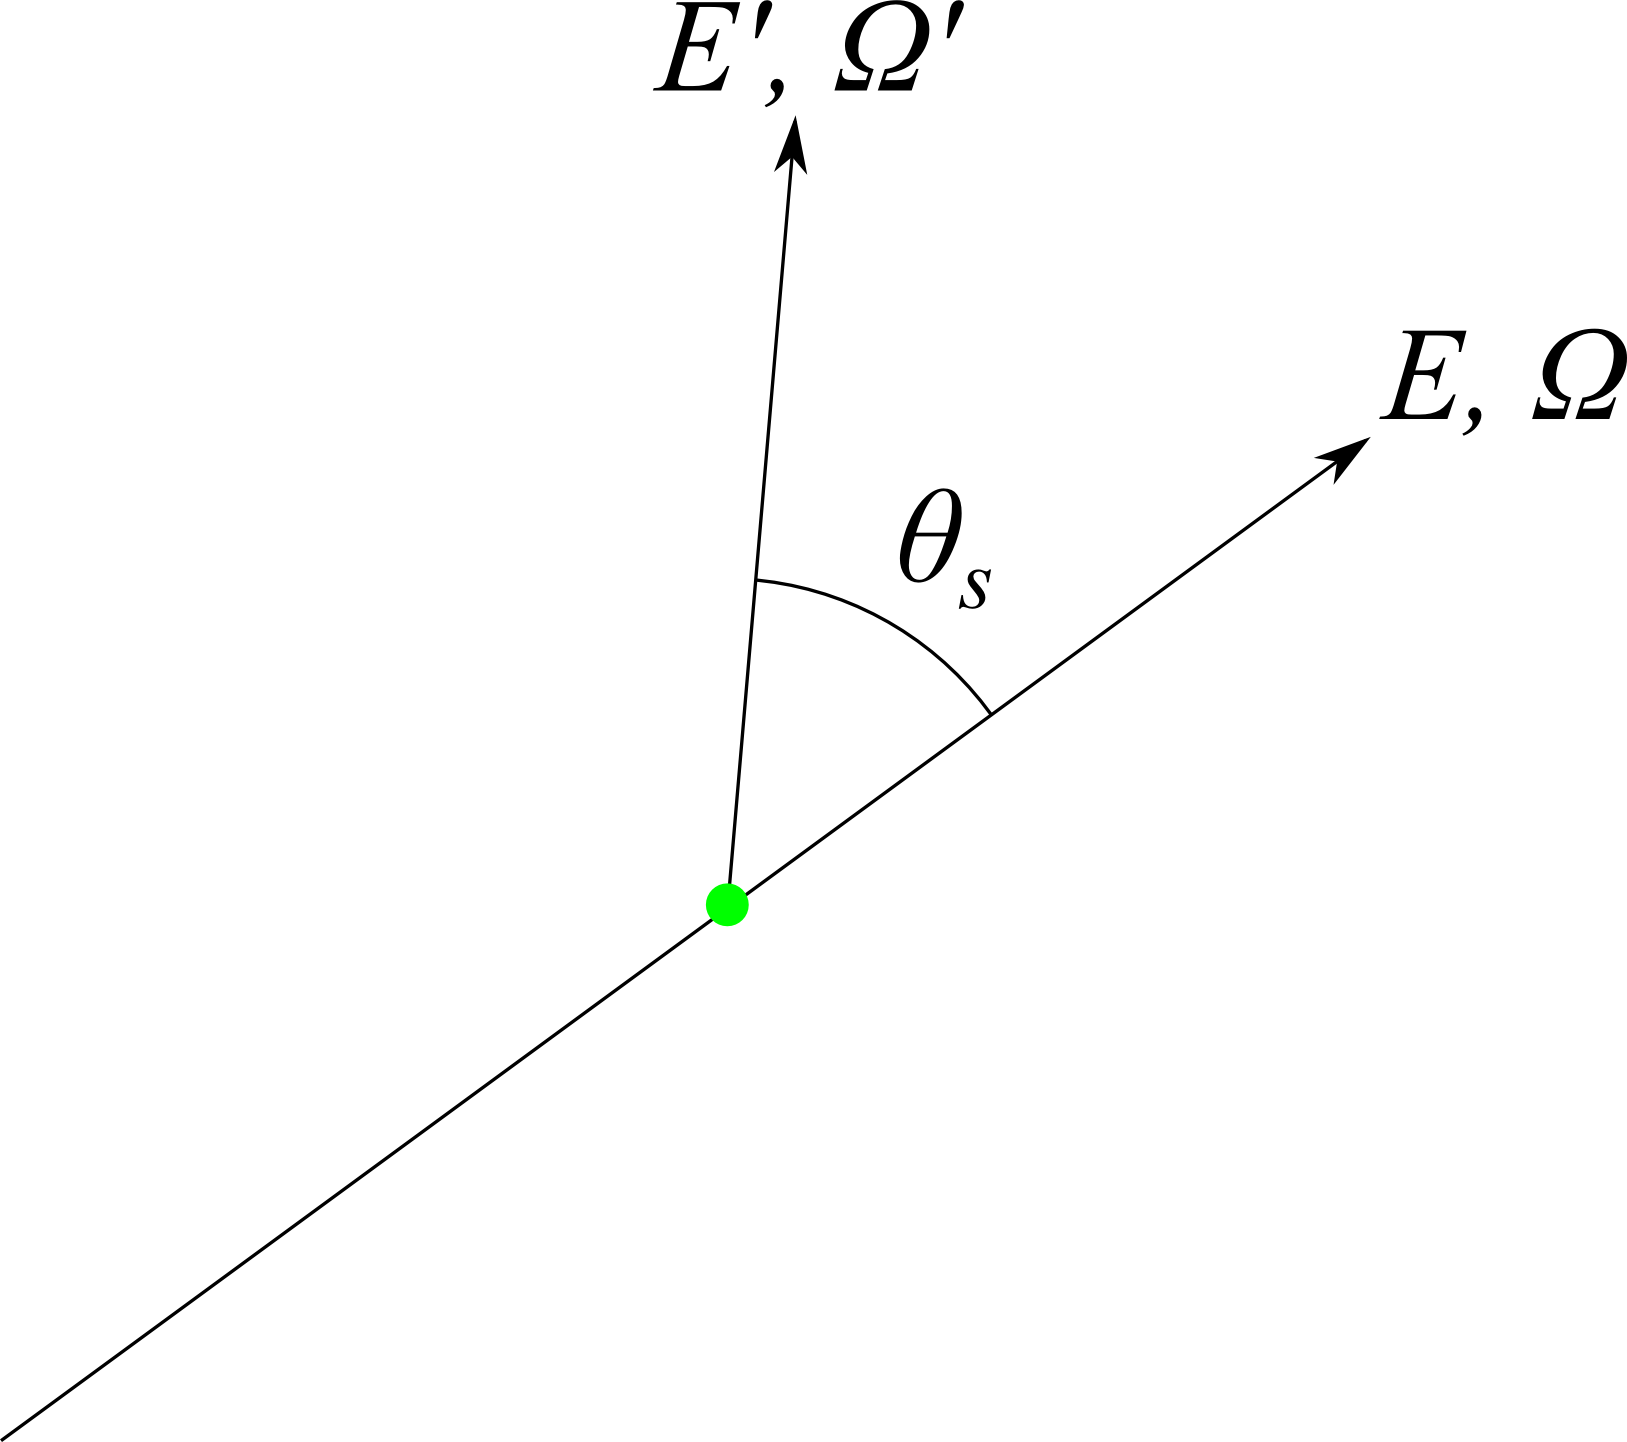
\includegraphics[width=3.75in]{figs/scat_ang}
  \end{center}
  \caption{The scatter angle. A photon at energy $E$ traveling in direction $\Omega$, hits a stationary atom, indicated by the green circle, and scatters into a new direction $\Omega'$ with a new energy $E'$.}
\label{fig:scat_ang}
\end{figure}%

The data files containing the scatter cross sections are distributed using a Legendre polynomial expansion. The use of a Legendre expansion removes the dependence on the quadrature from the data. This allows any quadrature to work with any dataset. A $l$-order Legendre polynomial is donoted by $P_l$. The anisotropic scatter cross section can then be rewritten as a Legendre expansion given in Eq.~\ref{eq:leg_1} where the scatter cosine is defined in Eq.~\ref{eq:scat_cos}

\begin{equation} \label{eq:leg_1}
\Sigma_{s, i, a, a'}^{g, g'} = \sum_{l=0}^L \frac{2l+1}{4 \pi}\Sigma_{s, i, l}^{g, g'} P_l(\mu_s)
\end{equation}

\begin{equation} \label{eq:scat_cos}
\mu_s = \Omega_a \cdot \Omega_{a'}
\end{equation}

\section{Uncollided Flux}
To avoid ray effect, the flux is split into collided and uncollided components as shown in Eq.~\ref{eq:totflux}. Equation~\ref{eq:boltz} can be rewritten as two equations solving for the uncollided flux, $\psi_u$, and collided flux, $\psi_c$ independently. Equation~\ref{eq:unc} has no scatter term since scattered particles are not considered in the uncollided flux. The source term, $S_u$, in Eq.~\ref{eq:col} is the first collision source.

\begin{equation} \label{eq:totflux}
\psi = \psi_u + \psi_c
\end{equation}

\begin{equation} \label{eq:unc}
\left[ \hat{\Omega} \cdot \nabla + \Sigma_t(\boldsymbol{r}, E) \right]
\psi_u(\boldsymbol{r}, E, \hat{\Omega}) =  S(\boldsymbol{r}, E, \hat{\Omega})
\end{equation}

\begin{equation} \label{eq:col}
\begin{split}
	&\left[ \hat{\Omega} \cdot \nabla + \Sigma_t(\boldsymbol{r}, E) \right]
	\psi_c(\boldsymbol{r}, E, \hat{\Omega}) = \\
	&\int_{4 \pi} \int_0^\infty \Sigma_s(\boldsymbol{r}, E' \rightarrow E, \hat{\Omega}' \rightarrow \hat{\Omega}) \psi_c(\boldsymbol{r}, E', \hat{\Omega}') dE' d\hat{\Omega}' + S_{u}(\boldsymbol{r}, E, \hat{\Omega})
\end{split}
\end{equation}

The uncollided flux in Eq.~\ref{eq:unc} can be analytically solved. The solution is given in Eq.~\ref{eq:uncsol} for a known isotropic point source located at position $\boldsymbol{s}$. The $\delta$ symbol in Eq.~\ref{eq:uncsol} is the Kronecker delta given by Eq.~\ref{eq:kronecker}. 

\begin{equation} \label{eq:uncsol}
\psi_u(\boldsymbol{r}, E, \hat{\Omega}) = 
S(\boldsymbol{s}, E)
\frac{e^{-\sum_i \Sigma_{t,i} x_i}}{4\pi |\boldsymbol{r}-\boldsymbol{s}|^2}
\delta\left( \hat{\Omega}, \frac{\boldsymbol{r}-\boldsymbol{s}}{|\boldsymbol{r}-\boldsymbol{s}|^2}\right)
\end{equation}

\begin{equation} \label{eq:kronecker}
\delta(\vec{A}, \vec{B}) = 
\begin{cases}
1, \quad \mathrm{if} \ \vec{A}=\vec{B} \\
0, \quad \mathrm{otherwise}
\end{cases}
\end{equation}

Equation~\ref{eq:uncsol} can be expanded to accomodate any number of spatially distributed sources of arbitrary directionality given in Eq.~\ref{eq:uncsol2} by integrating over the entire spatial domain, $V$.

\begin{equation} \label{eq:uncsol2}
\psi_u(\boldsymbol{r}, E, \hat{\Omega}) = \iiint_{V}
S(\boldsymbol{s}, E, \hat{\Omega})
\frac{e^{-\sum_i \Sigma_{t,i} x_i}}{|\boldsymbol{r}-\boldsymbol{s}|^2}
\delta\left( \hat{\Omega}, \frac{\boldsymbol{r}-\boldsymbol{s}}{|\boldsymbol{r}-\boldsymbol{s}|^2}\right)
d \boldsymbol{s}
\end{equation}

The uncollided source term, $S_u$ in Eq.~\ref{eq:col} is computed from the uncollided flux using Eq.~\ref{eq:uncsrc}.

\begin{equation} \label{eq:uncsrc}
S_u(\boldsymbol{r}, E, \hat{\Omega}) = \int_{4\pi} \int_{0}^{\infty} 
\Sigma_s(\boldsymbol{r}, E' \rightarrow E, \hat{\Omega}' \rightarrow \hat{\Omega}) \psi_u(\boldsymbol{r}, E', \hat{\Omega}') 
dE' d\hat{\Omega}'
\end{equation}

Substituting Eq.~\ref{eq:uncsrc} into $S_u$ in Eq.~\ref{eq:col} gives Eq.~\ref{eq:col2} which simplifies to Eq.~\ref{eq:col3} by using Eq.~\ref{eq:totflux} to replace the collided and uncollided components with the total angular flux.

\begin{equation} \label{eq:col2}
\begin{split}
	&\left[ \hat{\Omega} \cdot \nabla + \Sigma_t(\boldsymbol{r}, E) \right]
	\psi_c(\boldsymbol{r}, E, \hat{\Omega}) = \\
	&\int_{4 \pi} \int_0^\infty \Sigma_s(\boldsymbol{r}, E' \rightarrow E, \hat{\Omega}' \rightarrow \hat{\Omega}) \psi_c(\boldsymbol{r}, E', \hat{\Omega}') dE' d\hat{\Omega}' + \\
	&\int_{4\pi} \int_{0}^{\infty} 
\Sigma_s(\boldsymbol{r}, E' \rightarrow E, \hat{\Omega}' \rightarrow \hat{\Omega}) \psi_u(\boldsymbol{r}, E', \hat{\Omega}') 
dE' d\hat{\Omega}'
\end{split}
\end{equation}

\begin{equation} \label{eq:col3}
\begin{split}
	&\left[ \hat{\Omega} \cdot \nabla + \Sigma_t(\boldsymbol{r}, E) \right]
	\psi_c(\boldsymbol{r}, E, \hat{\Omega}) = \\
	&\int_{4 \pi} \int_0^\infty \Sigma_s(\boldsymbol{r}, E' \rightarrow E, \hat{\Omega}' \rightarrow \hat{\Omega}) \psi(\boldsymbol{r}, E', \hat{\Omega}') dE' d\hat{\Omega}'
\end{split}
\end{equation}

\section{Source Generation}
There are many kinds of external sources implemented in this work.

\subsection{Point Source}
The simplest source implemented is an isotropic point source. This source is defined only by its position and energy distribution. The center of the cell whose flux is being computed is located at position $<C_x, C_y, C_z>$ and the point source is located at position $<S_x, S_y, S_z>$.

\subsection{Fan Source}
In addition to the values defining a point source (position $\vec{S}$ and the energy distribution) a fan source is defined by two additional parameters, $\varphi$ and $\theta$ which describe the azimuthal and polar angles subtented by the fan beam respectively. Figure~\ref{fig:fanbeam} shows $\varphi$ and $\theta$ in reference to the geometry setup. The raytracing algorithm used for the fan beam is identical to the point source raytracer except for one difference: before the raytracing is done, whether the ray falls within the fan beam is determined and any ray falling outside the fan beam is not traced, its uncollided flux is immediately set to zero.

Some voxels would be partially enclosed inside the beam. A partial acceptance value is computed for these voxels and multiplied by the final result of the raytrace.

\begin{figure}[tb]
  \begin{center}
   \includegraphics[width=3.75in]{figs/fan_rejection}
  \end{center}
  \caption{The fan.}
\label{fig:fan_rejection}
\end{figure}

First, the ray direction is projected onto the $xy$ plane giving $<S_x, S_y, 0>$ and $C_x, C_y, 0$. Then the vector from the source to the geometry center and the vector from the source to the cell center are dotted to give the cosine of the angle between them as shown in Eq.~\ref{eq:phicos}. Once $\zeta$ is computed, the condition given by Eq.~\ref{eq:phicoscon} is evaluated. If the condition is met, the angle is accepted and raytraced normally, otherwise, it is rejected immediately. Figure~\ref{fig:phi}

\begin{figure}[tb]
  \begin{center}
   \includegraphics[width=3.75in]{figs/phi}
  \end{center}
  \caption{How $\varphi$ is computed.}
\label{fig:phi}
\end{figure}

\begin{equation}\label{eq:phicos}
\cos(\zeta_\varphi) = \frac{<S_x, S_y, 0>}{\sqrt{S_x^2 + S_y^2}} \cdot \frac{<C_x, C_y, 0>}{\sqrt{C_x^2 + C_y^2}} = \frac{S_x C_x + S_y C_y}{\sqrt{S_x^2 + S_y^2} \sqrt{C_x^2 + C_y^2}}
\end{equation}

\begin{equation}\label{eq:phicoscon}
|\zeta_\varphi| < \frac{\varphi}{2}
\end{equation}

Treatment for the $\theta$ variable is similar to that of $\varphi$ except the polar angle is required instead of the azimuthal angle. This is computed using Eq.~\ref{eq:thetacos} for an arbitrary vector $\vec{\xi}$. This is used to compute the polar angle for both $\vec{S}$ and $\vec{C}$. The difference between the polar angles of the two vectors is computed using Eq.~\ref{eq:thetacos2} and then the condition given in Eq.~\ref{eq:thetacoscon} is evaluated. If the condition is not met, the ray is rejected and no raytrace is performed.

\begin{equation}\label{eq:thetacos}
\cos(\theta_\xi) = \frac{\xi_z}{\sqrt{\xi_z^2 + \xi_y^2 + \xi_z^2}}
\end{equation}

\begin{equation}\label{eq:thetacos2}
\zeta_\theta = \theta_S - \theta_C
\end{equation}

\begin{equation}\label{eq:thetacoscon}
|\zeta_\theta| < \frac{\vartheta}{2}
\end{equation}


\subsection{Multi-fan Source}
A focal point is determined. The focal spot is at the center of each fan beam. The focal spot is always assumed to be at the center of the geometry and at the same $z$ elevation as the source point.

\begin{figure}
    \centering
    \begin{subfigure}[b]{0.2\textwidth}
        \includegraphics[width=\textwidth]{figs/proj6}
        \caption{$N=6$}
        \label{fig:proj6}
    \end{subfigure}
    ~ %add desired spacing between images, e. g. ~, \quad, \qquad, \hfill etc. 
      %(or a blank line to force the subfigure onto a new line)
    \begin{subfigure}[b]{0.2\textwidth}
        \includegraphics[width=\textwidth]{figs/proj12}
        \caption{$N=12$}
        \label{fig:proj12}
    \end{subfigure}
    ~ %add desired spacing between images, e. g. ~, \quad, \qquad, \hfill etc. 
    %(or a blank line to force the subfigure onto a new line)
    \begin{subfigure}[b]{0.2\textwidth}
        \includegraphics[width=\textwidth]{figs/proj16}
        \caption{$N=16$}
        \label{fig:proj16}
    \end{subfigure}
    \begin{subfigure}[b]{0.2\textwidth}
        \includegraphics[width=\textwidth]{figs/proj24}
        \caption{$N=24$}
        \label{fig:proj24}
    \end{subfigure}
    \caption{Different numbers of fan beam projections.}\label{fig:fanproj}
\end{figure}

\begin{equation}\label{eq:xp}
x' = x \cos \theta - y \sin \theta
\end{equation}

\begin{equation}\label{eq:yp}
y' = y \cos \theta + x \sin \theta
\end{equation}

To rotate a point $(x,y)$ about an arbitrary point $(x_f, y_f)$, Eq.~\ref{eq:xp2} and~\ref{eq:yp2} are used.

\begin{equation}\label{eq:xp2}
x' = (x-x_f) \cos \theta - (y-y_f) \sin \theta + x_f
\end{equation}

\begin{equation}\label{eq:yp2}
x' = (y - y_f) \cos \theta + (x - x_f) \sin \theta + y_f
\end{equation}

\subsection{Cone Source and Multi-cone Source}
Cone sources are identical to fan beam sources except for the rejection criteria used to determine whether or not a voxel is inside the beam. The rejection crieria is a function of only a single parameter, $\theta$, the maximum permissible angle between the center of the beam and a ray toward the point of interest.

The actual angle is $\zeta$ which is computed similarly to Eq.~\ref{eq:phicos} without the projection onto the $xy$ plane in Eq.~\ref{eq:zetacos} can be simplified to a simple summation since both $\vec{S}$ and $\vec{C}$ are unit vectors.

\begin{equation}\label{eq:zetacos}
\cos(\zeta) = \frac{<S_x, S_y, S_z>}{\sqrt{S_x^2 + S_y^2 + S_z^2}} \cdot \frac{<C_x, C_y, C_z>}{\sqrt{C_x^2 + C_y^2 + C_z^2}} = S_x C_x + S_y C_y + S_z C_z
\end{equation}

\begin{equation}\label{eq:zetacon}
|\zeta| < \theta
\end{equation}

\begin{figure}
    \centering
    \begin{subfigure}[b]{0.45\textwidth}
        \includegraphics[width=\textwidth]{figs/beamconexy}
        \caption{Cone xy}
        \label{fig:beamconexy}
    \end{subfigure}
    ~
    \begin{subfigure}[b]{0.45\textwidth}
        \includegraphics[width=\textwidth]{figs/beamfanxy}
        \caption{Fan xy}
        \label{fig:beamfanxy}
    \end{subfigure}

    \begin{subfigure}[b]{0.45\textwidth}
        \includegraphics[width=\textwidth]{figs/beamconeyz}
        \caption{Cone yz}
        \label{fig:subsweep_general3}
    \end{subfigure}
    ~
    \begin{subfigure}[b]{0.45\textwidth}
        \includegraphics[width=\textwidth]{figs/beamfanyz}
        \caption{Fan yz}
        \label{fig:subsweep_general4}
    \end{subfigure}
    
    \begin{subfigure}[b]{0.45\textwidth}
        \includegraphics[width=\textwidth]{figs/beamconexz}
        \caption{Cone xz}
        \label{fig:subsweep_general5}
    \end{subfigure}
    ~
    \begin{subfigure}[b]{0.45\textwidth}
        \includegraphics[width=\textwidth]{figs/beamfanxz}
        \caption{Fan xz}
        \label{fig:subsweep_general6}
    \end{subfigure}
    \caption{The beam shapes.}\label{fig:beamfancone}
\end{figure}


\subsection{Multileaf Collimator}
How fancy.

Talk about the MCNP generation in the comparison to results part.

\endinput
%%
%% End of file `chapmin.tex'.
